\documentclass[11pt]{article}
\usepackage[margin=0.85in]{geometry}
\usepackage{amsmath,amssymb}
\usepackage{tikz}
\usepackage{fancyhdr}
\usepackage[hidelinks]{hyperref}
\pagestyle{fancy}\fancyhf{}
\fancyhead[L]{PHYS 3316: Quantum Mechanics}
\fancyhead[R]{WKB approximation}
\fancyfoot[C]{\thepage}
\setlength{\headheight}{14pt}
\setlength{\parindent}{0pt}
\setlength{\parskip}{6pt}
\newcommand{\dd}{\,\mathrm{d}}
\begin{document}
\begin{center}
{\Large\bfseries The WKB Approximation in One Dimension}\\[4pt]
{\large Slowly varying potentials, tunneling, and alpha decay}\\[3pt]
November 17, 2026
\end{center}

\section*{1. The physical idea: a local wavelength}
For a constant potential, the time-independent Schr\"odinger equation has plane-wave solutions. If the potential changes slowly, we expect a wave whose wavelength changes gradually with position.
\begin{equation}
-\frac{\hbar^2}{2m}\psi''(x)+V(x)\psi(x)=E\psi(x).
\end{equation}
In a classically allowed region, define
\begin{equation}
p(x)=\sqrt{2m[E-V(x)]},\qquad
k(x)=\frac{p(x)}{\hbar},\qquad
\lambda(x)=\frac{2\pi\hbar}{p(x)}.
\end{equation}
The phase accumulated over a small displacement is $\dd\phi=k(x)\dd x$. Thus the natural replacement for $kx$ is $\int^x k(x')\dd x'$.

\textbf{Question for the class:} If a particle moves into a region with larger $V(x)$, what happens to its momentum and wavelength? What should happen to the probability density for a fixed transmitted current?

\section*{2. Deriving the WKB wavefunction}
Write the wavefunction as a slowly varying amplitude times a rapidly varying phase:
\begin{equation}
\psi(x)=A(x)e^{iS(x)/\hbar}.
\end{equation}
Differentiating twice gives
\begin{equation}
\psi''=e^{iS/\hbar}\left[A''+\frac{i}{\hbar}(2A'S'+AS'')
-\frac{A(S')^2}{\hbar^2}\right].
\end{equation}
Substituting into the Schr\"odinger equation,
\begin{equation}
\left[\frac{(S')^2}{2m}+V-E\right]A
-\frac{i\hbar}{2m}(2A'S'+AS'')-\frac{\hbar^2}{2m}A''=0.
\end{equation}
At leading order, neglect $A''$. Taking $A$ and $S$ real in an allowed region, the real part gives
\begin{equation}
S'=\pm p(x),\qquad S(x)=\pm\int^x p(x')\dd x'.
\end{equation}
The imaginary part gives $2pA'+p'A=0$, or
\begin{equation}
\frac{A'}{A}=-\frac{p'}{2p},\qquad A(x)\propto\frac{1}{\sqrt{p(x)}}.
\end{equation}

\newpage
\section*{3. Allowed and forbidden regions}
The two independent allowed-region solutions are
\begin{equation}
\boxed{\psi(x)\approx\frac{1}{\sqrt{p(x)}}
\left[C_+e^{\frac{i}{\hbar}\int^x p(x')\dd x'}
+C_-e^{-\frac{i}{\hbar}\int^x p(x')\dd x'}\right].}
\end{equation}
The lower integration limit is any fixed reference point in the region; changing it only changes the constants' phases.

\textbf{Why does the amplitude depend on momentum?} For either traveling component,
\begin{equation}
j=\frac{\hbar}{m}\operatorname{Im}(\psi^*\psi')
=\pm\frac{|C_\pm|^2}{m}.
\end{equation}
The factor $1/\sqrt p$ keeps the current constant. Equivalently, $|\psi|^2\propto1/p\propto1/v$: the density is greater where the particle moves more slowly.

In a classically forbidden region, $V(x)>E$, define a positive quantity with units of momentum,
\begin{equation}
q(x)=\sqrt{2m[V(x)-E]}.
\end{equation}
The WKB solutions become exponential:
\begin{equation}
\boxed{\psi(x)\approx\frac{1}{\sqrt{q(x)}}
\left[D_+e^{\frac{1}{\hbar}\int^x q(x')\dd x'}
+D_-e^{-\frac{1}{\hbar}\int^x q(x')\dd x'}\right].}
\end{equation}
For a finite barrier, both terms generally occur in the matched solution. A single decaying exponential describes the dominant attenuation but carries no probability current by itself.

\section*{4. When does the approximation work?}
The local momentum should change little over a distance $\hbar/p$:
\begin{equation}
\boxed{\frac{\hbar|p'(x)|}{p(x)^2}\ll1.}
\end{equation}
An analogous condition holds with $q$ in a forbidden region. More directly, the derivation requires $\hbar^2|A''|\ll p^2|A|$ in the allowed region.

At a \textbf{turning point}, $V(x_t)=E$ and $p(x_t)=0$. The WKB amplitude diverges, so the approximation fails locally. The physical wavefunction remains finite. For a smooth, simple turning point, a local Airy-function solution connects the allowed and forbidden solutions. We will use the resulting tunneling estimate without deriving these connection formulas.

\textbf{Takeaway:} Oscillatory where $E>V$; exponential where $E<V$; special matching is needed near $E=V$.

\newpage
\section*{5. Tunneling through a barrier}
Suppose a smooth barrier has two turning points $x_1$ and $x_2$, with $V(x)>E$ between them. Define the dimensionless barrier integral
\begin{equation}
K=\frac{1}{\hbar}\int_{x_1}^{x_2}\sqrt{2m[V(x)-E]}\dd x.
\end{equation}
The wave amplitude is attenuated by approximately $e^{-K}$, and the leading transmission probability for an opaque barrier ($K\gg1$) is
\begin{equation}
\boxed{T\approx e^{-2K}
=\exp\left[-\frac{2}{\hbar}\int_{x_1}^{x_2}\sqrt{2m[V(x)-E]}\dd x\right].}
\end{equation}
Here $T=j_{\mathrm{trans}}/j_{\mathrm{inc}}$. Matching fixes any prefactor. The expression is not reliable near the barrier top, where $K$ is small.

\subsection*{Worked example: a rectangular barrier}
Let $V(x)=V_0$ for $0<x<a$ and zero outside, with $0<E<V_0$. Although the discontinuous boundaries require exact matching, the same attenuation argument gives the leading exponential:
\begin{equation}
\kappa=\frac{\sqrt{2m(V_0-E)}}{\hbar},\qquad
\boxed{T\sim e^{-2\kappa a}.}
\end{equation}
For an electron,
\begin{equation}
\kappa=5.12\,\mathrm{nm}^{-1}\sqrt{\frac{V_0-E}{\mathrm{eV}}}.
\end{equation}
If $V_0-E=1.0\,\mathrm{eV}$ and $a=0.50\,\mathrm{nm}$, then
\begin{equation}
2\kappa a=5.12,\qquad T\sim e^{-5.12}\approx6.0\times10^{-3}.
\end{equation}
Doubling the width gives $T(2a)\sim[T(a)]^2\approx3.6\times10^{-5}$.

\textbf{Optional comparison with exact matching.} For equal potentials on both sides,
\begin{equation}
T_{\mathrm{exact}}=
\left[1+\frac{V_0^2\sinh^2(\kappa a)}{4E(V_0-E)}\right]^{-1}.
\end{equation}
For $\kappa a\gg1$,
\begin{equation}
T_{\mathrm{exact}}\approx\frac{16E(V_0-E)}{V_0^2}\,e^{-2\kappa a}.
\end{equation}
The attenuation estimate captures the exponential dependence; it does not determine the rectangular barrier's boundary prefactor.

\textbf{Discussion:} A wider barrier, a higher barrier, or a heavier particle suppresses tunneling exponentially. The exponent depends on the entire forbidden region, not only the maximum barrier height.

\newpage
\section*{6. Application: alpha-particle decay}
An alpha particle is confined by the attractive nuclear interaction at short distance. Outside the nuclear surface it experiences repulsion from the daughter nucleus. It can have positive escape energy while remaining trapped behind a Coulomb barrier.

For zero orbital angular momentum, the reduced radial wavefunction $u(r)=r\psi(r)$ obeys a one-dimensional Schr\"odinger equation on $r>0$:
\begin{equation}
-\frac{\hbar^2}{2\mu}u''(r)+V(r)u(r)=Eu(r),\qquad
\mu=\frac{m_\alpha M_d}{m_\alpha+M_d}.
\end{equation}
Use a simple model with a nuclear well inside radius $R$ and, outside,
\begin{equation}
V(r)=\frac{C}{r},\qquad
C=\frac{2Z_de^2}{4\pi\epsilon_0},\qquad Z_d=Z-2.
\end{equation}
Here $E$ is the kinetic energy of relative alpha--daughter motion at infinity (including daughter recoil), not just the alpha's laboratory kinetic energy. Assume $0<E<C/R$. The outer turning point is
\begin{equation}
\boxed{b=\frac{C}{E}.}
\end{equation}
The surface $R$ approximates the inner edge of the barrier in this model.

\begin{center}
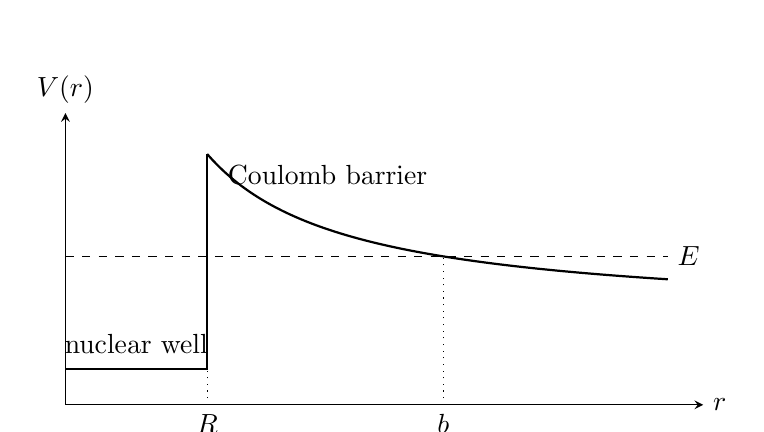
\begin{tikzpicture}[x=0.9cm,y=0.65cm,>=stealth]
\draw[->] (0,-1.7)--(9,-1.7) node[right] {$r$};
\draw[->] (0,-1.7)--(0,4) node[above] {$V(r)$};
\draw[thick] (0,-1)--(2,-1)--(2,3.2);
\draw[thick,domain=2:8.5,samples=80] plot (\x,{6.4/\x});
\draw[dashed] (0,1.2)--(8.5,1.2) node[right] {$E$};
\draw[dotted] (2,-1.7)--(2,3.2);
\draw[dotted] (5.333,-1.7)--(5.333,1.2);
\node[below] at (2,-1.7) {$R$};
\node[below] at (5.333,-1.7) {$b$};
\node at (3.7,2.8) {Coulomb barrier};
\node at (1,-0.5) {nuclear well};
\end{tikzpicture}
\end{center}
The leading tunneling probability per collision with the barrier is
\begin{equation}
\boxed{T\approx\exp\left[-\frac{2}{\hbar}
\int_R^b\sqrt{2\mu\left(\frac{C}{r}-E\right)}\dd r\right].}
\end{equation}
\textbf{Physical point:} Classical escape is impossible at this energy, but the forbidden region has finite width, so quantum escape has nonzero probability.

\newpage
\section*{7. From barrier penetration to a half-life}
Let $\rho=R/b$. With the substitution $r=b\sin^2\theta$, the barrier integral becomes
\begin{align}
\int_R^b\sqrt{2\mu(C/r-E)}\dd r
&=2b\sqrt{2\mu E}\int_{\sin^{-1}\sqrt\rho}^{\pi/2}\cos^2\theta\dd\theta\\
&=b\sqrt{2\mu E}
\left[\cos^{-1}\sqrt\rho-\sqrt{\rho(1-\rho)}\right].
\end{align}
Therefore,
\begin{equation}
\boxed{-\ln T\approx\frac{2b\sqrt{2\mu E}}{\hbar}
\left[\cos^{-1}\sqrt{R/b}-\sqrt{(R/b)(1-R/b)}\right].}
\end{equation}
For $R/b\ll1$, the bracket is $\pi/2-2\sqrt{R/b}+O((R/b)^{3/2})$, giving
\begin{equation}
-\ln T\approx\frac{\pi C\sqrt{2\mu}}{\hbar\sqrt E}
-\frac{4\sqrt{2\mu CR}}{\hbar}+\cdots.
\end{equation}
The dominant energy dependence is proportional to $Z_d/\sqrt E$.

\subsection*{Collision frequency and decay rate}
Let $f_{\mathrm{coll}}$ denote the \textbf{collision frequency}: how often the alpha particle collides with the nuclear barrier. In a simple traversal model,
\begin{equation}
f_{\mathrm{coll}}\sim\frac{v_{\mathrm{in}}}{2R},
\end{equation}
where $v_{\mathrm{in}}$ is its speed inside the nuclear well. For a well of depth $V_N>0$ measured relative to zero outside, $v_{\mathrm{in}}\approx\sqrt{2(E+V_N)/\mu}$.

If the alpha is already formed and each collision has small escape probability $T$, then
\begin{equation}
\lambda\approx f_{\mathrm{coll}}T,\qquad
N(t)=N(0)e^{-\lambda t},\qquad
\boxed{t_{1/2}=\frac{\ln2}{f_{\mathrm{coll}}T}.}
\end{equation}
A more realistic model includes an alpha-preformation probability $P_\alpha$, so $\lambda\approx P_\alpha f_{\mathrm{coll}}T$. Nuclear structure and nonzero angular momentum can also change the rate.

For related nuclei, treating the remaining factors as slowly varying gives the approximate \textbf{Geiger--Nuttall relation}
\begin{equation}
\boxed{\log_{10}\!\left(\frac{t_{1/2}}{1\,\mathrm{s}}\right)
\approx A\frac{Z_d}{\sqrt{E/\mathrm{MeV}}}+B.}
\end{equation}
The fitted constants depend on the nuclear family. A modest increase in decay energy can shorten the half-life by many orders of magnitude.

\textbf{Closing question:} Why can two nuclei with similar sizes and decay energies have vastly different half-lives? Identify the quantity in the WKB exponent that controls this sensitivity.
\end{document}
